\documentclass{ifacconf}

\usepackage{graphicx}      % include this line if your document contains figures
\usepackage{natbib}        % required for bibliography
\usepackage{listings}		% source code
\def\Section {\S}
%===============================================================================
\begin{document}
\begin{frontmatter}
%\title{ Decentralized Multi-robot Control\\ Using HEAD: Hybrid Event-driven Architecture on D-Bus   \thanksref{footnoteinfo}} 
%\title{ Flexible Multi-robot Control\\ Using HEAD: Hybrid Event-driven Architecture on D-Bus   \thanksref{footnoteinfo}} 
% Title, preferably not more than 10 words.
\title{Flexible Communication in Multi-robotic Control System Using HEAD: Hybrid Event-driven Architecture on~D-Bus   \thanksref{footnoteinfo}} 

\thanks[footnoteinfo]{This research has been funded by the Engineering and Physical Sciences Research Council (EPSRC), UK, grant reference EP/E061915/1.}

\author{Md Omar Faruque Sarker and } 
\author{Torbj{\o}rn S. Dahl.} 

\address{Robotic Intelligence Lab, University of Wales, Newport\\
Allt-yr-yn Campus, Allt-yr-yn Avenue, Newport, NP205DA, UK\\
 (e-mail: Mdomarfaruque.Sarker|Torbjorn.Dahl@newport.ac.uk)}

\begin{abstract}                % Abstract of not more than 250 words.
Direct real-time communication among various software components of a multi-robot system (MRS) is much more complicated than that in software simulations. Existing inter-process communication (IPC) mechanisms, such as pipes, shared memory etc., are very rigid and usually enforce tight coupling among software components. Thus they do not integrate well with heterogeneous multi-robot control applications of a relatively larger MRS that typically consists of tens of robots and various sensing and monitoring elements interconnected through several host PCs. In this paper, we present a modular, flexible and decentralized multi-robot control architecture, namely hybrid event-driven architecture on D-Bus (HEAD), that overcomes these issues by decoupling IPC through D-Bus. D-Bus is a relatively new IPC technology for modern Linux desktop environments. It typically uses a message bus daemon that facilitates asynchronous data sharing among multiple processes. Here, we show that by using only a single type of message, namely D-Bus {\em signal} type, HEAD can efficiently enable real-time interactions among heterogeneous multi-robot control applications. The design of HEAD is flexible enough to add various types of existing and new software components with minimum programming effort. As an example, we present how we achieve a decentralized peer-to-peer communication behaviours among robot controller clients by simply adding only a few lines of new code leaving the major IPC implementation intact. This paper also reports the performance of D-Bus, under both constant and variable IPC load, obtained from our MRS implementation of a manufacturing shop-floor scenario with 16 e-puck robots.
\end{abstract}

\begin{keyword}
multi-robot system, real-time control, inter-process communication, D-Bus
%Five to ten keywords, preferably chosen from the IFAC keyword list.
\end{keyword}

\end{frontmatter}
%===============================================================================
\section{Introduction}
Inter-process communications (IPC) among various desktop software components enable them to talk to each other and exchange data, messages or request of services. Technological advancements in computer and communication systems now allow robotic researchers to set-up and conduct experiments on multi-robot systems (MRS) from desktop PCs. Many compelling reasons, including open licensing model, availability of open-source tools for almost free of cost, community support etc., make Linux as an ideal operating system for MRS research. However the integration of heterogeneous software components in Linux desktop becomes a challenging issue, particularly when each robot-control software needs sensory and other data input from various other software components (e.g. pose data from a tracker server, task information from a task server etc).\\ 
Traditional IPC solutions in a standard Linux desktop, e.g. pipes, sockets, X atoms, shared memory, temporary files etc. (hereafter called {\em traditional IPCs}), are too static and rigid to meet the demand of a dynamic software system (\cite{wittenburg2005}). On the other hand, complex and heavy IPC like CORBA fails to integrate into a development tool-chain efficiently. They also require a steep learning curve due to their complex implementations. Besides, the failure of Desktop Communication Protocol (DCOP) in system-wide integration and interoperability issues encouraged the development of the D-Bus message bus system, D-Bus for short (\cite{Pennington+2010}). This message bus system provides simple mechanisms for applications to talk to one another (see details in Section 2). In this paper we describe  how we exploit the simplicity and power of D-Bus  for running a large MRS.\\
%%
Our work has been undertaken as part of a collaborative EPSRC (UK) funded project ``Defying the Rules: How Self-Regulatory Social Systems Work” where we have studied the behaviour of ants, humans and robots and have developed the attractive field model (AFM), a common formal model of division of labour in social systems (\cite{Arcaute+2008}). In our part, our on-going research aims to validate AFM by exploring different communication models in a MRS having about 40 E-puck robots.  Existing MRS research, such as in swarm robotics, IPC among a large group of robots (more than 10) are rare. Most of the robotic researchers either use a simulation platform or a small group of robots with no or limited direct communication (e.g., \cite{Labella2007}).   However in our research, we have emphasized the use of real robotic systems so that we can gain practical insight about the limitations and state-of-the art in multi-robot communication systems.\\
%%
In pursuing a suitable multi-robot control architecture for our large number of robots, we have found that traditional IPCs are inadequate to support the important requirements of IPC among several heterogeneous software components of a large MRS. Firstly, real-time support in IPC is critical for connecting time-critical control applications. For example, a multi-robot tracking system (MRTS) can share robot pose information with a robot-controller client (RCC) though shared memory (SHM). This pose information can be used to help navigating a robot in real-time. However if MRTS crashes and stops writing new pose information into the SHM, RCC has no default mechanism to know that SHM data is outdated. Some form of reference counting mechanism can be used to overcome this issue, but that makes the implementation of RCC complicated and error-prone.\\
Secondly, IPC must be scalable so that adding more software components (thus more robots, sensors, etc.) in the information sharing game does not affect the overall system performance. But clearly this can not be achieved through traditional IPCs, e.g. SHM or temporary files,  as the access to computer memory and disk space is costly and time consuming. Thirdly, IPC should be flexible and compatible enough to allow existing software components to join with newly developed components in the information sharing without much difficulties. Again existing IPC mechanisms are too static and rigid to be integrated with existing software components. Besides, incompatibility often arises among different applications written in different programming languages with different semantics of IPC. Fourthly, IPC should be robust, fault-tolerant and loosely coupled so that if one ceases to work others can still continue to work without strange runtime exceptions. Finally, IPC should be implemented simply and efficiently in any modern high level programming languages, e.g., C/C++, Java, Python etc. Practically this is very important since IPC will be required in many places of code and application programmers have little time to look inside the detail implementation of any IPC.\\
%%
Here we present a scalable and distributed multi-robot control architecture built upon D-Bus IPC. D-Bus IPC works asynchronously in real-time. It has virtually no limit how many software components participate in information sharing. In fact, to the best of our knowledge, the performance of D-Bus daemon does not vary if the number of participating software components varies. In this paper we have shown that by using only the signalling interfaces, SwisTrack (\cite{Lochmatter+2008}), an open-source multi-robot tracking tool can be integrated with our multi-robot control framework. All software components are loosely coupled and unlike traditional IPCs, one does not depend on another for setting up and shutting down IPC infrastructure. For example, in case of SHM one software component explicitly needs to set-up and clean-up SHM spaces. In case of D-Bus any software component can join and leave in the information sharing process at any time. Each component implements its own fall-back strategy if desired information from another component is unavailable at any time. Based on a thin C API, D-Bus also provides many binding in common programming languages. In this work, we use {\em dbus-python}, a Python binding for D-Bus, that provide us a very clean and efficient IPC mechanism.\\
%%
Rest of this paper is organized as follows. Section~\ref{sec:dbus} presents an overview of DBus IPC technology.  Section~\ref{sec:head} describes our multi-robot control architecture HEAD with its design and characteristics, D-Bus communication interfaces and flexible communication schemes.  Section~\ref{sec:impl} reports an implementation of HEAD including the interactions between the hardware, software and communication modules. It also includes  our experimental results of D-Bus communication load. Section~\ref{sec:conc} draws conclusions.
%===============================================================================
\section{D-Bus Communication Model}
\label{sec:dbus}
%%%%%%%%%%%%%%%%%%
\subsection{D-Bus Overview}
D-BUS was designed from scratch to replace CORBA and DCOP  to fulfil the needs of a modern Linux system. D-BUS can perform basic application IPC as well as it can facilitate sending events, or signals, through the system, allowing different components in the system to communicate. D-BUS is unique from other IPC mechanisms in several ways, e.g. 1) the basic unit of IPC in D-BUS is a message, not a byte stream, 2) D-BUS is bus-based and 3) It has separate system-wide and user/session-wide bus (\cite{Love2005}) . The simplest form of D-Bus communication is process to process. However, it provides a daemon, known as the message bus daemon, that routes messages between processes on a specific bus. In this fashion, a bus topology is formed (see Fig. \ref{fig:dbus-daemon}), allowing processes to speak to one or more applications at the same time. Applications can send to or listen for various events on the bus.\\
D-Bus specification (\cite{Pennington+2010}) provides full details of D-Bus message protocols, message and data types, implementation guidelines and so forth. Here we discuss some relevant part of this specification. As we have already mentioned D-Bus provides a system-wide system bus and user-level session bus. Fig. \ref{fig:dbus-daemon} an example of this bus structure. In this paper we have limited our discussion to the latter one and skipped some advance topics like D-Bus security and so on.
%%
\begin{figure}
\begin{center}
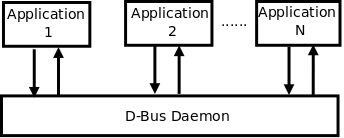
\includegraphics[width=7cm,height=3.1cm]{./dia-files/dbus-daemon} % The printed column width is 8.4 cm.
\caption{A typical view of D-Bus message bus system } 
\label{fig:dbus-daemon}
\end{center}
\end{figure}
%%
Here a few basic D-Bus terminologies have been introduced from D-Bus literature.\\
\textbf{D-Bus Connection: }
\textit{DBusConnection} is the structure that a program first uses to initiate talking to the D-Bus daemon, Programs can either use DBUS\_BUS\_SYSTEM or DBUS\_BUS\_SESSION to talk to the respective daemons.\\
\textbf{DBus Message: }
It is simply a message between two process. All the DBus intercommunication are done using \textit{DBusMessage}. These messages can have the following four types: method calls, method returns, signals, and errors. The DBusMessage structure can carry data payload, by appending boolean integers, real numbers, string, arrays, etc. to the message body.\\ 
\textbf{D-Bus Path: }
This is the path of a remote \textit{Object} (hereafter, this is captitalized to avoid ambiguity) of target process, e.g. \/org\/freedesktop\/DBus.\\
\textbf{D-Bus Interface: }
This is the interface on a given Object to talk with, e.g. org.freedesktop.DBus.\\
\textbf{D-Bus Method Call: }
This is a type of DBus message that used to invoke a method on a remote Object.\\
\textbf{D-Bus Signal: }
This is a type of DBus message to make a signal emission. As stated in D-Bus specification, Signal messages must have three header fields: PATH giving the object the signal was emitted from, plus INTERFACE and MEMBER giving the fully-qualified name of the signal. The INTERFACE header is required for signals, though it is optional for method calls. The structure of a signal is shown Fig. \ref{fig:dbus-signal-protocol} and it shows the design of robot-status signal that emits over specified interfaces and paths with a data payload of an integer and a string containing robot-status message.\\
\textbf{D-Bus Error: }
This is the structure that holds the error code which occurs by calling a DBus method.
%%
\begin{figure}
\begin{center}
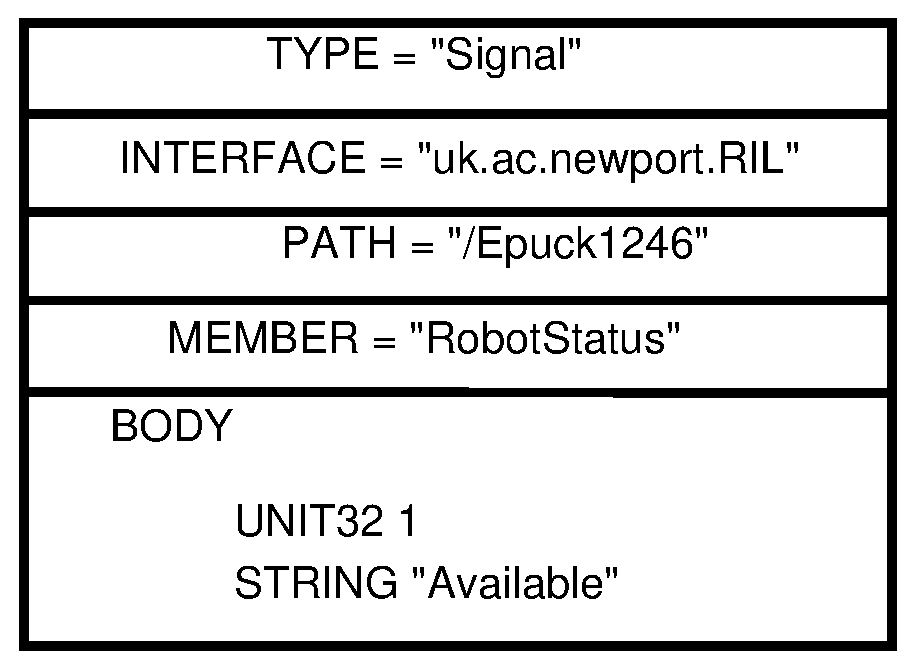
\includegraphics[width=5cm,height=4cm]{./dia-files/dbus-signal-protocol} % The printed column width is 8.4 cm.
\caption{A typical structure of a D-Bus signal message} 
\label{fig:dbus-signal-protocol}
\end{center}
\end{figure}
%%%%%%%%%%%%%%%%%%
\subsection{Strategies for Application Integration}
Under D-Bus, there are two basic mechanisms for applications to interact with each other: by calling a remote Object of target application and by emitting a signal for interested applications. To perform a method call on a D-BUS Object, a method call message must be sent to that Object. It will do some processing and return either a method return message or an error message. Signals are different in that they cannot return anything: there is neither a "signal return" message, nor any other type of error message see this \footnote{http://www.ibm.com/developerworks/linux/library/l-dbus.html} for some example use-cases. Thus on D-Bus everything can be done asynchronously without the need of polling.\\ 
D-Bus provides several language bindings for integrating D-Bus to any native application. The core D-BUS API, written in C, is rather low-level and large. On top of this API, bindings integrate with programming languages and environments, including Glib, Python, Qt and Mono. On top of providing language wrappers, the bindings provide environment-specific features. For example, the Glib bindings treat D-BUS connections as GObjects and allow messaging to integrate into the Glib mainloop. The preferred use of D-BUS is definitely using language and environment-specific bindings, both for ease of use and improved functionality (\cite{Love2005}).
%===============================================================================
\section{Hybrid Event-driven Architecture on D-Bus (HEAD)}
\label{sec:head}
%%%%%%%%%%%%%%%%%%
\subsection{Overview of Multi-robot Control}
Controlling a robot in a well-organized manner involves following a control architecture. As defined by \cite{Mataric2007}, a robot control architecture is a set of guiding principles and constraints for organizing a robot's control system. Since last few decades, robot control architectures has been evolving from deliberative to reactive and hybrid (combination of deliberative and reactive), behaviour-based and to some other forms. It has been well established that hybrid control can bring together the best aspects of both reactive and deliberative control by combining the real-time low-level device control and high-level deliberative action control. Only reactive (or deliberative) control approach is not enough for enabling robots to do complex tasks in a dynamic environments (\cite{Gat1997}).\\
 As shown in Fig. \ref{fig:three-layer-arch}, this is usually achieved by a three-layer architecture composed of deliberator, sequencer and controller . Controller usually works under real-time reactive feedback control loops to do simple tasks by producing primitive robot behaviours, e.g. obstacle avoidance, wall following etc. Deliberator performs time-consuming computations, e.g. running exponential search or computer vision processing algorithms. In order to achieve specific task goals, the middle component, sequencer, typically integrates both deliberator and controller maintaining consistent, robust and timely robot behaviours.\\
%%%
\begin{figure}
\begin{center}
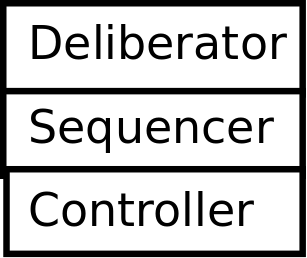
\includegraphics[width=2.5cm,height=2.1cm]{./dia-files/three-layer-arch} % The printed column width is 8.4 cm.
\caption{Classical three layer robot control architecture after (\cite{Gat1997})} 
\label{fig:three-layer-arch}
\end{center}
\end{figure}
%%%%%%%%%%%%%%%%%%
\subsection{Characteristics of {\em HEAD}}
%%
\begin{figure}
\begin{center}
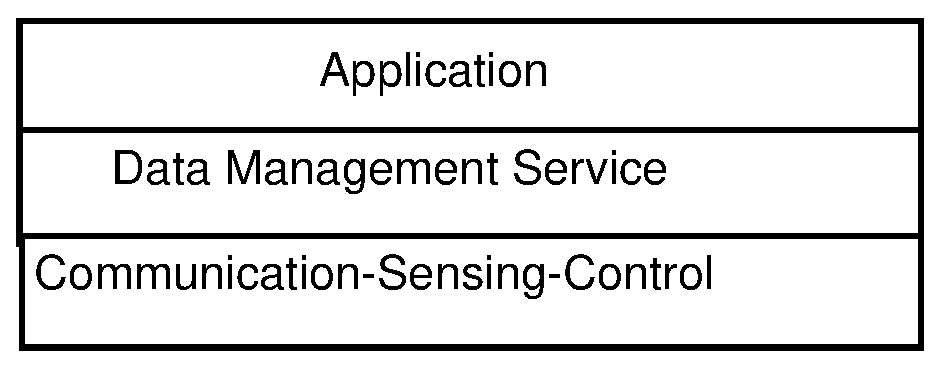
\includegraphics[width=5.5cm,height=2.1cm]{./dia-files/abstract-arch} % The printed column width is 8.4 cm.
\caption{Our abstract multi-robot control architecture} 
\label{fig:abstract-arch}
\end{center}
\end{figure}
We organized our  multi-robot control architecture, HEAD into three layers as shown in Fig. \ref{fig:abstract-arch}. Although HEAD has been designed by adopting the principles of hybrid architecture it has many distinct features that are absent in a classical hybrid architecture. Firstly, with respect to controller layer, HEAD broadly views sensing and control as communication with external entities. Communication as sensing is not new, e.g. it has been reported in multi-agent learning (\cite{Mataric1998}) and many other places. When robots' on-board computing resources are limited communication can effectively make up their required sensing capabilities. On the other hand, low-level device control is also a series of communication act where actuator commands are typically transmitted over a radio or physical link. Thus, at the bottom layer of HEAD is the communication layer where all external communication takes place over any suitable medium. Components sitting in this layer either act as sensors that can receive environmental state, task information, self pose data etc. via suitable communication link or do the real-time control of devices by sending actuator commands over a target communication channel. \\
Secondly, the apparent tight coupling with sensors to actuators has been reduced by introducing a data and event management (DEM) layer. DEM acts as a short-term storage of sensed data and various events posted by both controller and deliberator components. Task sequencing has been simplified by automated event triggering mechanism. DEM simply creates new event channels and interested components subscribe to this event for reading or writing. If one components updates an event DEM updates subscribed components about this event. Controller and deliberator components synchronize their tasks based on this event signals. DEM efficiently serves newly arrived data to controller and deliberator components by this event mechanism. Thus neither specialized languages are needed to program a sequencer nor cumbersome if/else checks are present in this layer.\\
Finally, deliberator layer of HEAD has been described as an application layer that runs real-application code based on high-level user algorithms as well as low-level sensor data and device states. In classic hybrid architecture the role of this layer has been described mainly in two folds: 1) producing task plan and sending it to sequencer and 2) answering queries made by sequencer. Application layer of HEAD follows the former one by generating plan and queuing it to DEM layer, but it does not support the latter one. DEM layer never makes a query to an application since it acts only as a passive information gateway. Thus this reduced coupling between DEM and application layer has enhanced HEAD with additional robustness and scalability. Additional applications can be added with DEM layer's existing or new event interfaces. Any malfunction or failure in application layer or even in communication layer can be isolated without affecting others. 
%%
\begin{figure*}
\begin{center}
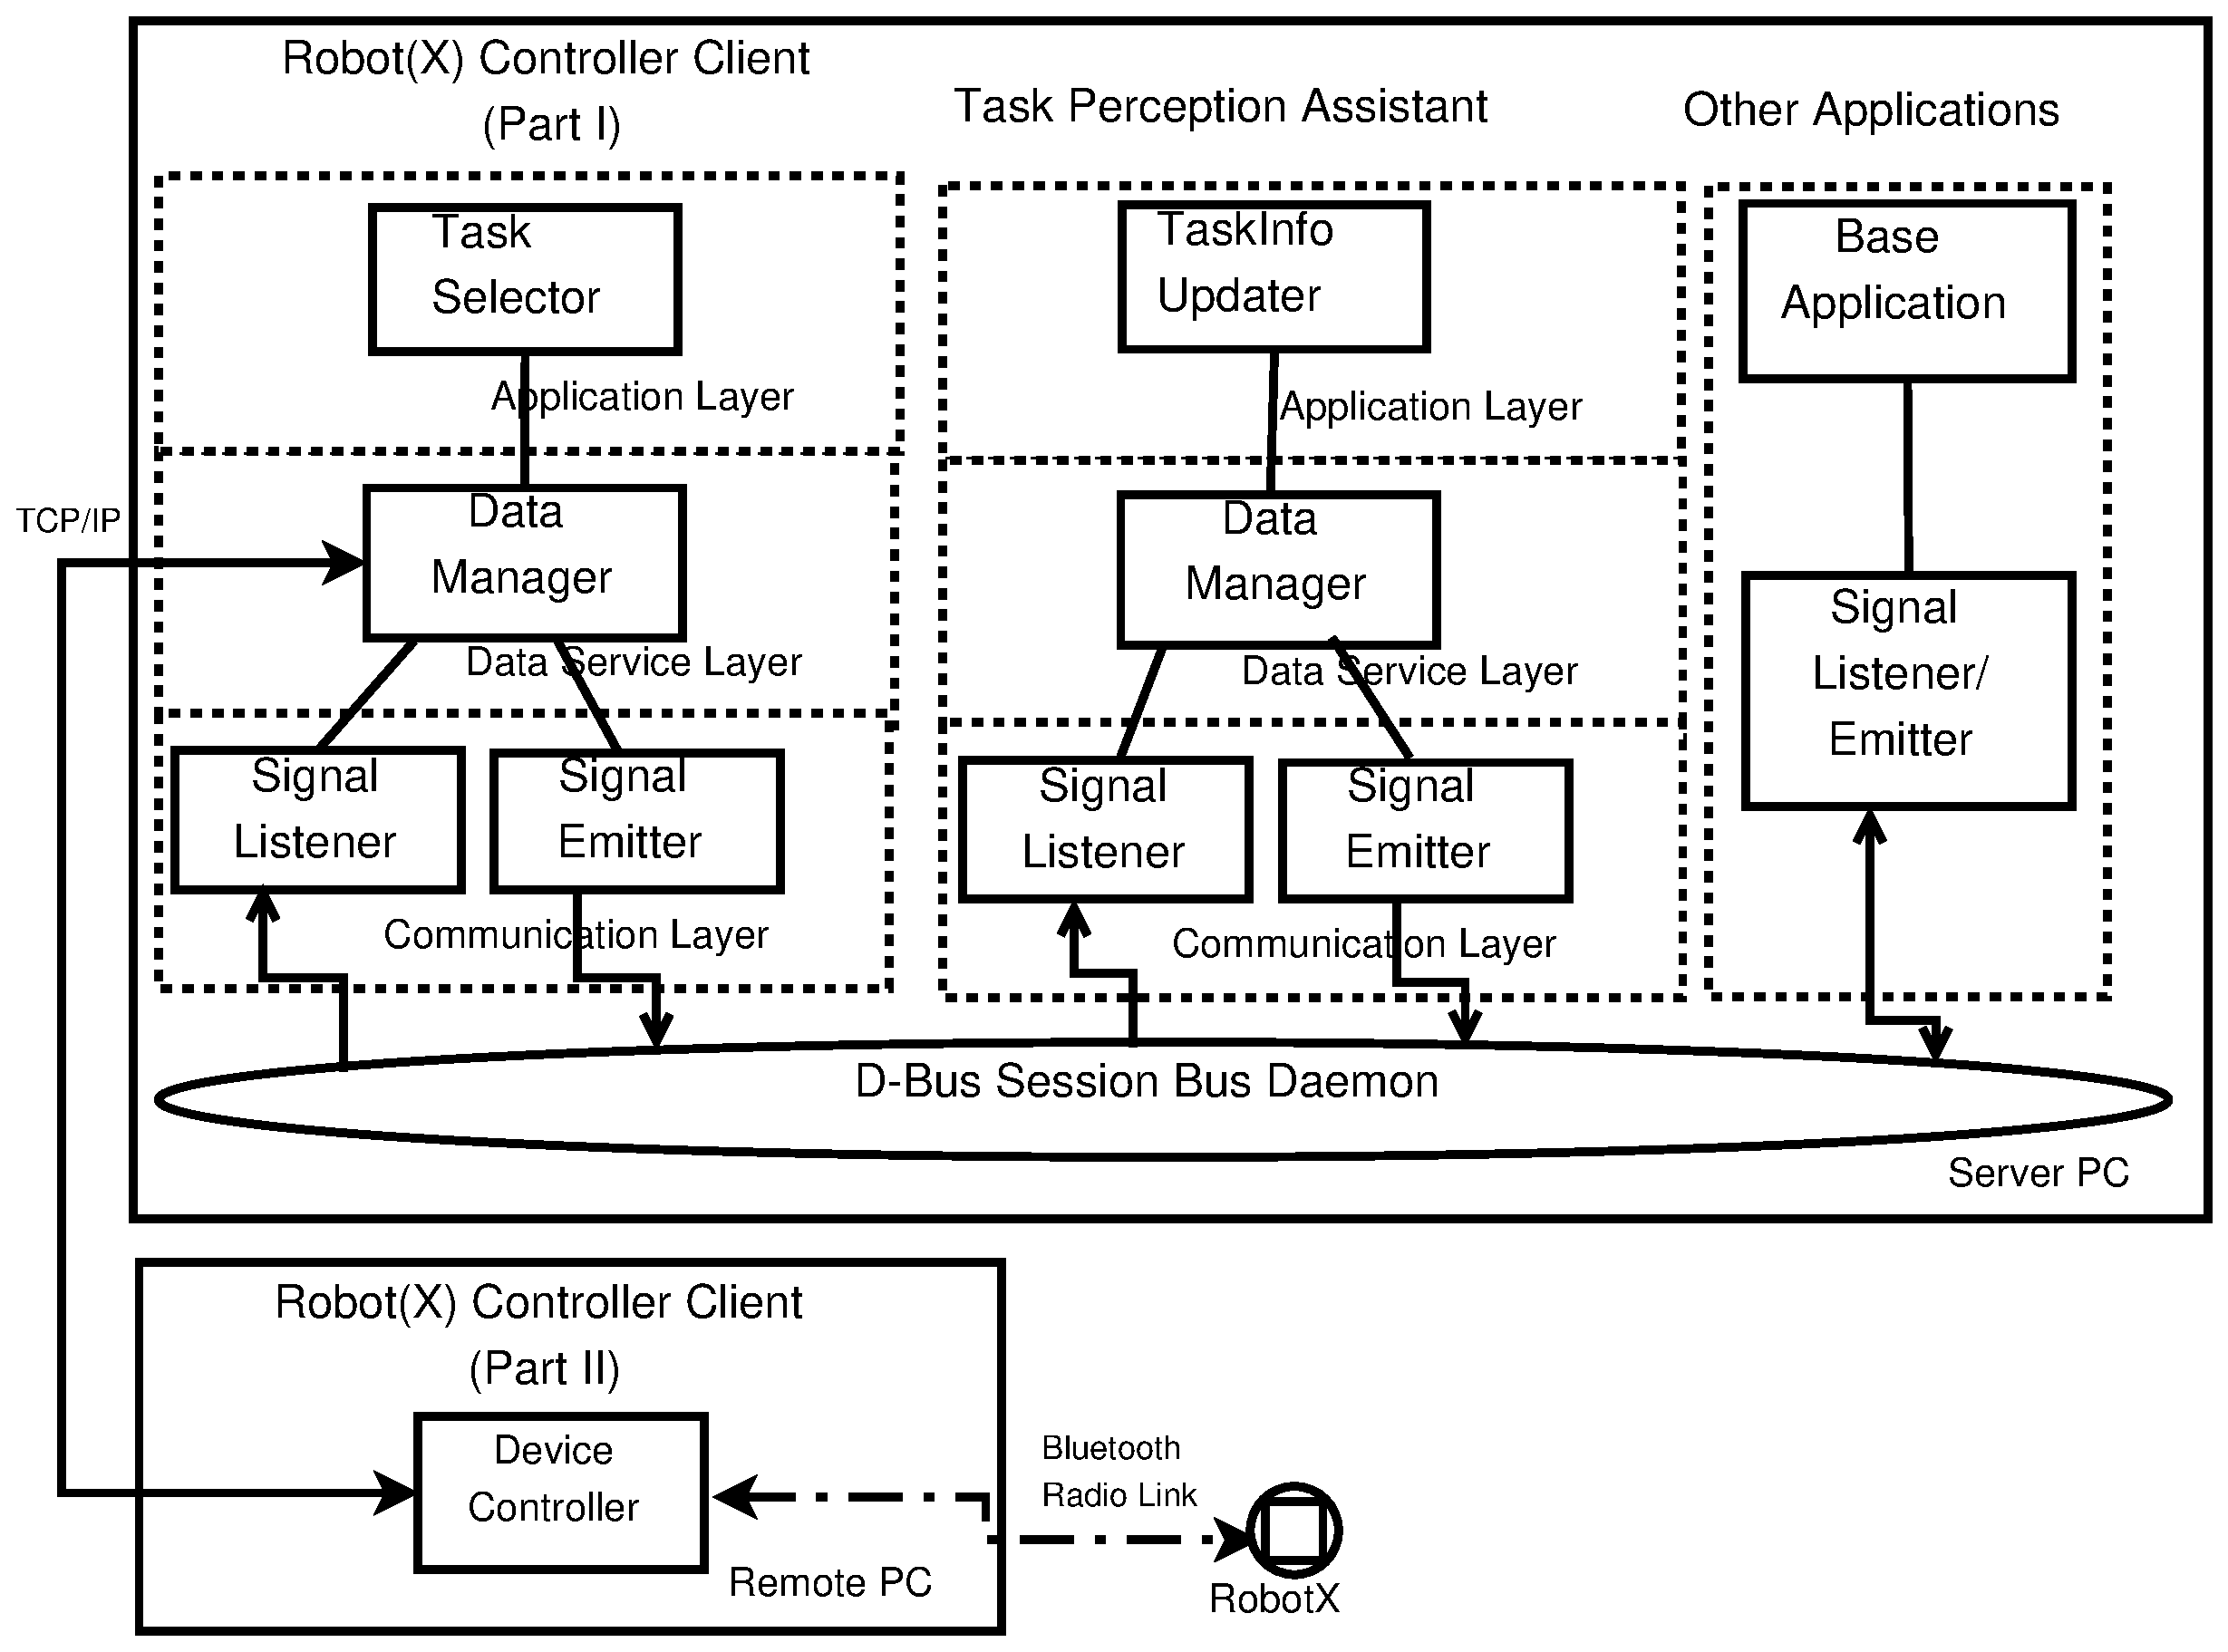
\includegraphics[width=12cm,height=8cm]{./dia-files/concrete-arch} % The printed column width is 8.4 cm.
%\centering
\caption{General outline of {\em HEAD}. Robot-Controller-Client application has been splitted into two parts: one runs locally in server PC and another runs remotely, e.g., in embedded PC} 
\label{fig:concrete-arch}
\end{center}
\end{figure*}
%%%%%%%%%%%%%%%%%%
\subsection{D-Bus Signal Interfaces and Software Integrations}
D-Bus IPC allows us to completely decouple the interaction of different parts of software components of HEAD. Here we use the term {\em software component} or application to denote the logical groupings of several sub-processes or threads that works under a mother process or main thread (here we use the term thread and process interchangeably). Software components that follows our three-layer architecture for grouping its processes are called {\em native component} whereas existing software applications are called {\em external component}. As shown in Fig. \ref{fig:concrete-arch}, RCC and TPA are native software components of HEAD whereas SwisTrack, a multi-robot tracking tool (\cite{Lochmatter+2008}) used with HEAD, is called an external component.\\
In order to integrate both native and external components with HEAD. We have designed two separate communication process: a D-Bus signal reception process, SignalListener, and a D-Bus signal emission process, SignalEmitter. Inside a native component both of this process can communicate with data and event management process, DataManager, by using any suitable mechanisms, such as, multi-threading, multi-processing (offered in Python multiprocessing \footnotetext{http://docs.python.org/library/multiprocessing.html}), TCP or any other networking protocol.\\
Any external component that intend to act as a sensing (actuating) element of HEAD need to implement a SignalEmitter (SignalListener). For example, we extend SwisTrack with D-Bus signal emitting code (aka SignalEmitter) so that it can emit robot pose messages to individual robots D-Bus path under a common interface (uk.ac.newport.SwisTrack). This emitted signal is then caught by SignalListener of individual robot's RCC. Thus the tight-coupling between SwisTrack and RCC has been removed. During run-time SwisTrack can flexibly track variable number of robots and broadcast their corresponding pose messages without any re-compilation of code. Moreover, in worse cases, if SwisTrack or RCC crashes it does not affect any other component at run-time.\\
Expanding SignalEmitter and SignalListener for more D-Bus signals does not require to make any change the IPC implementation code. Let us first look at how to setup a signal emission process.

\textbf{Steps for setting up signal emission:}\\
\textbf{Step 1:} Connect to a D-Bus daemon. Sample C code:
\lstset{language=C,basicstyle=\small}
\begin{lstlisting}
DBusError error;
DBusConnection *conn;
dbus_error_init (&error);
conn = dbus_bus_get (DBUS_BUS_SESSION, &error);
\end{lstlisting}
\textbf{Step 2:} Optionally reserve a D-Bus path or service name (this is not required if the same path is not used by any other process).\\
\textbf{Step 3:} Send signal to a specified path. Sample C code:
\begin{lstlisting} 
DBusMessage *message;
message = dbus_message_new_signal (
``/target/dbus/path",``target.dbus.interface",
``Config");
/* Send the signal */
dbus_connection_send (connection, message, NULL);
dbus_message_unref (message);
\end{lstlisting}
%%
In order to add more signals we just need to repeat step 3 as many times as we need. On the other hand, signal listening can be done by setting up a suitable event loop under any supported language bindings. A basic implementation of both of these processes in Python language can be found in this tutorial \footnote{http://dbus.freedesktop.org/doc/dbus-python/doc/tutorial.html}. 
%%%%%%%%%%%%%%%%%%
%\subsection{Common Interfaces}
%	D-Bus Signal Listener
% 	D-Bus Signal Emitter
%===============================================================================
\subsection{Flexible Communication  Schemes}
%%%%%%%%%%%%%%%%%%
HEAD provides flexibility in designing communication among multiple components. By using a proper combination of signal interface and path different communication patterns can be achieved. For example, one component can broadcast signal S in interface A and path P and interested components can listen to this signal by matching to interface, path and signal. On the other hand for peer-to-peer (P2P) decentralized communication,  we give each application its own interface and different interacting nodes a separate path.  For example, if a multi-robot tracker intend to send individual robot pose to different RCCs, it can do that by using path P1,  P2, etc. under same S and A. Finally in case of each RCC intending to send signals to its neighbour RCCs, we design our signal emitter in a such a way that each RCC can listen signals coming to its own signal path but can emit  signal to other possible paths of the group. Thus,  this types of strategies  make it possible to avoid bouncing a signal to self and to simplify the overall testing and debugging of D-Bus communication of different applications in real-time. Moreover, D-Bus library comes with a handy tool, dbus-monitor, that can be used to listen to messages and debug the behaviours of applications.
%===============================================================================
\section{Implementation of a Multi-robot Manufacturing Scenario}
\label{sec:impl}
\begin{figure*}
\begin{center}
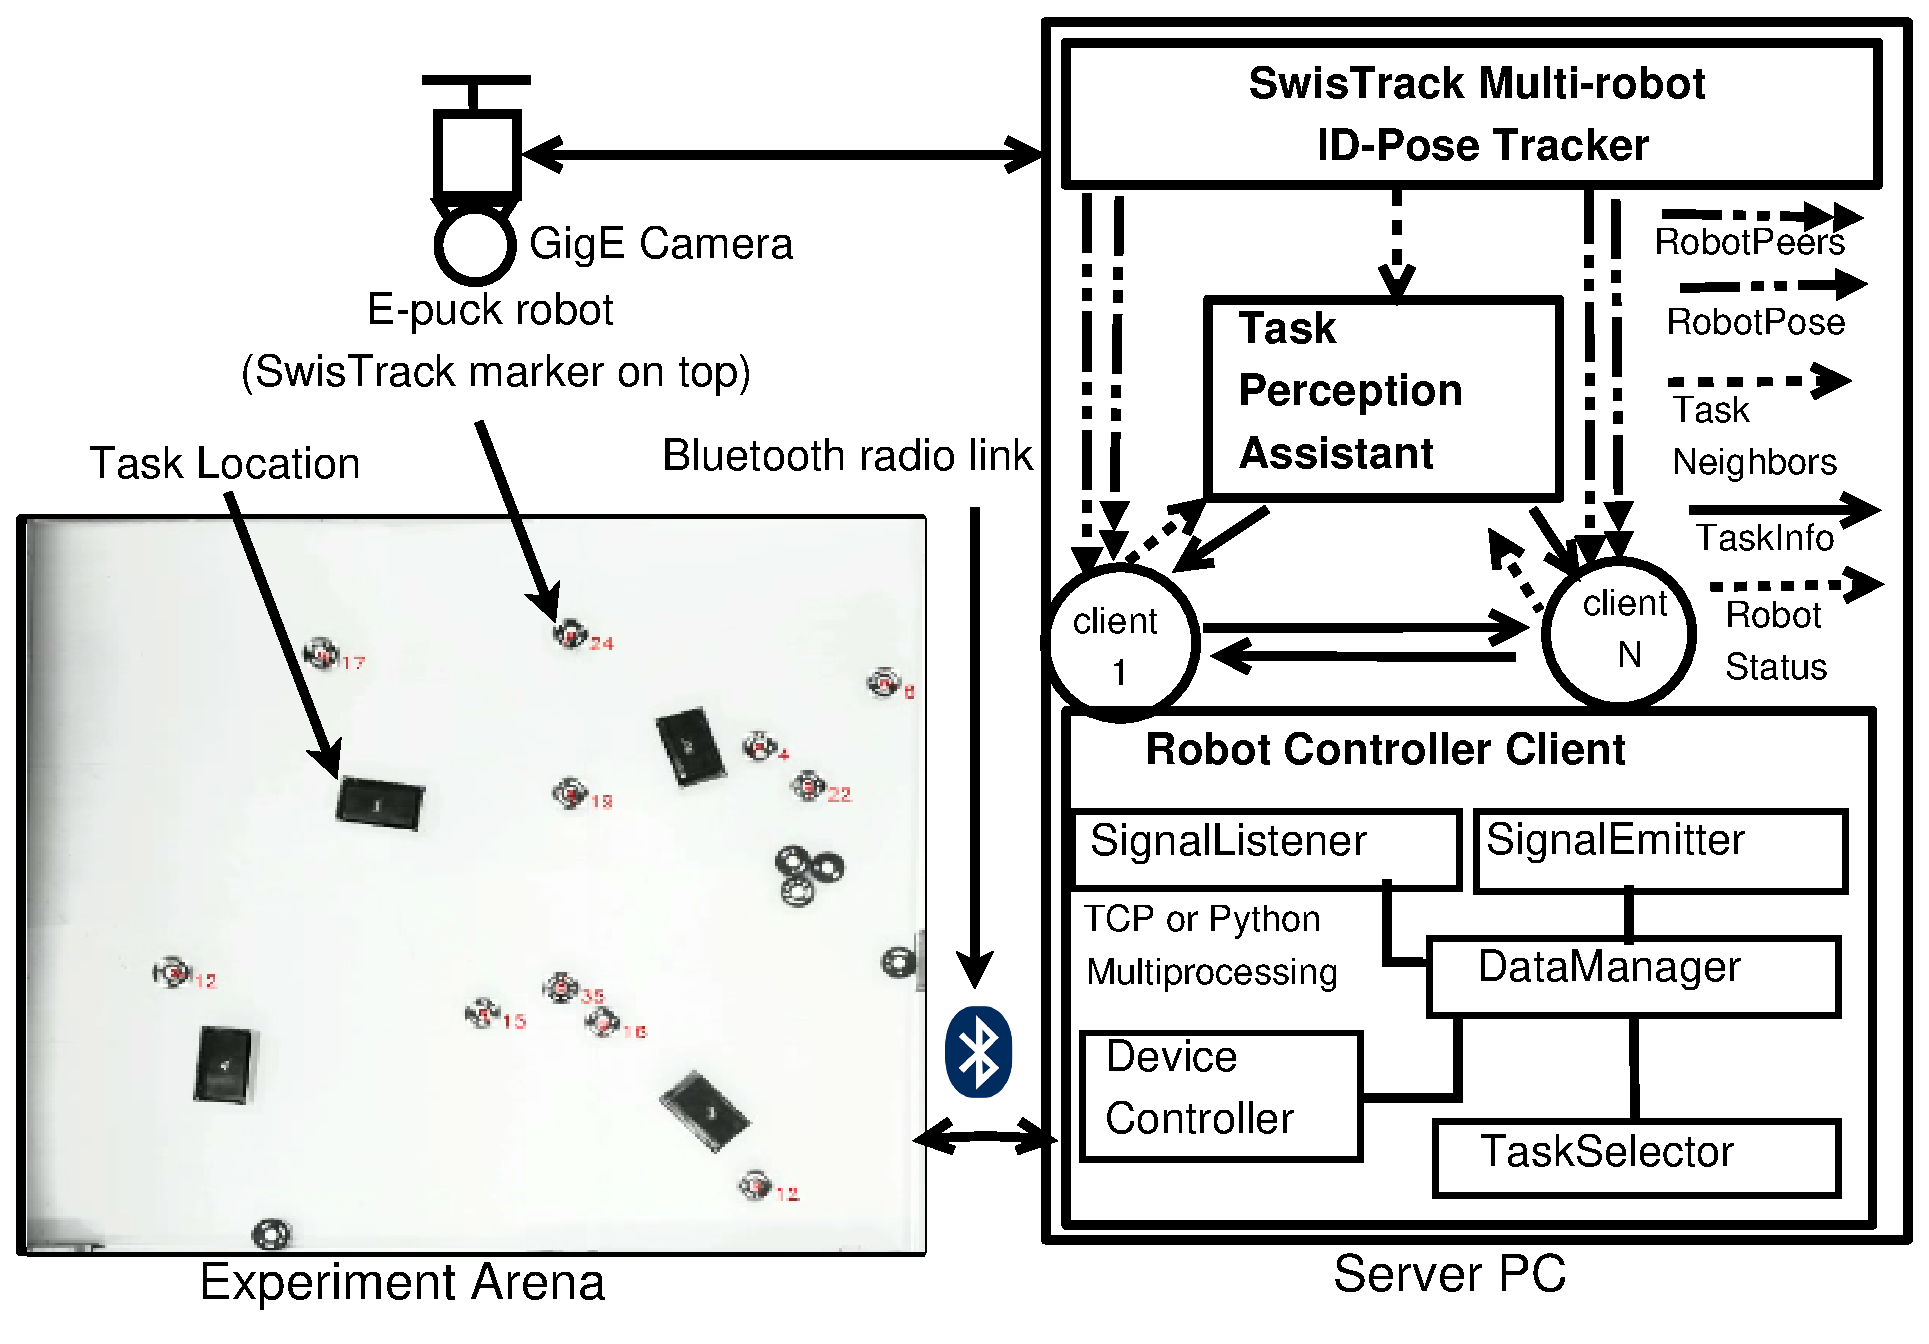
\includegraphics[width=12cm,height=7.5cm]{./dia-files/RIL-Expt-Setup3}    % The printed column width is 8.4 cm.
%\centering
\caption{An example implementation of {\em HEAD}. Various D-Bus signals are active in an automated loop (without any operator interaction). In decentralized communication mode RCCs can talk to each other and exchange task information through D-Bus signals} 
\label{fig:setup}
\end{center}
\end{figure*}
%%%%%%%%%%%%%%%%%%%%%%%%%%%%%%%%%%%%%%%%
\subsection{Multi-robot Task Allocation}
We have performed a multi-robot task allocation experiments in a manufacturing shop-floor scenario where N number of mobile robots are required to attend to M number of shop tasks spread over  fixed area A. Let these tasks be represented by a set of small rectangular boxes resembling to manufacturing machines. In order to complete a shop task $j$, a robot $R_i$ needs to reach within a fixed boundary $D_{j}$ . Each task $j$ has an associated task-urgency $\phi_j$ that indicates its relative importance over time. If a robot attends to a task $j$ in x$^{th}$ time-step, value of $\phi_j$ will decreases by a small amount $\delta_\phi$ in (x+1)$^{th}$ time-step. On the other hand, if a task has not been served by any robot in x$^{th}$ time-step, $\phi_j$ will increase by another small amount in (x+1)$^{th}$ time-step. According AFM, all robots will establish attractive fields to all tasks due to the presence of a system-wide continuous flow of information. The strength of these attractive fields called stimulus will vary according to the distances between robots and tasks, task-urgencies and corresponding sensitizations of robots etc. The detail mathematical model of each robot' task selection mechanism based on AFM and its robotic implementation can be found in (\cite{Arcaute+2008,Sarker+2010ants}).
%%%%%%%%%%%%%%%%%%%%%%%%%%%%
\subsection{Experiments}
We have developed a system where up to 40 E-puck\footnote{www.e-puck.org} robots can operate together according to the generic rules of the AFM. In \cite{Sarker+2010ants} we reported a set of experiments that were designed to validate AFM by testing the occurrence of convergent MRTA.  As shown in Fig. \ref{fig:setup} (right), our software system consists of a multi-robot tracking system, a task perception assistant (TPA) and robot controller clients (RCC). We have developed an IPC component for SwisTrack that can broadcast id and pose of all robots in real-time over our server's D-Bus interface.\\
Apart from SwisTrack, we have implemented two major software modules: {\em Task Perception Assistant (TPA)} and {\em Robot Controller Client (RCC)}. They are developed in Python with its state of the art \textit{Multiprocessing} \footnote{http://docs.python.org/library/multiprocessing.html} module. This python module simplifies our need to manage data sharing and synchronization among different sub-processes. As shown in Fig. \ref{fig:setup}, RCC consists of five sub-processes: {\em SignalListener} and {\em SignalEmitter}, interface with SwisTrack D-Bus Server and TPA. {\em DataManager} handles data storage and event management issues. {\em TaskSelector} implements AFM guidelines for task selection . {\em DeviceController} moves a robot to a target task. Bluetooth radio link is used as a communication medium between a RCC and a corresponding E-puck robot.  
%%%%%%%%%%%%%%%%%%%%%%%%%%%%%%%%%%%
\subsection{Results}
In our experiments, we recorded the D-Bus communication load on our communication system with varying level of task urgencies (see Fig. \ref{fig:task-urgency}) in both centralized and decentralized communication mode. In  centralized communication mode, communication load was almost constant over time (Fig. \ref{fig:global-freq}).  However in decentralized communication mode, since the emission of robot P2P signals happened asynchronously we found that the overall communication load on the system varied over time (Fig. \ref{fig:local-freq}). In Fig. \ref{fig:robot-freq} we see that a robot was able to listen a maximum of 9 P2P signals simultaneously.
\begin{figure}
\begin{center}
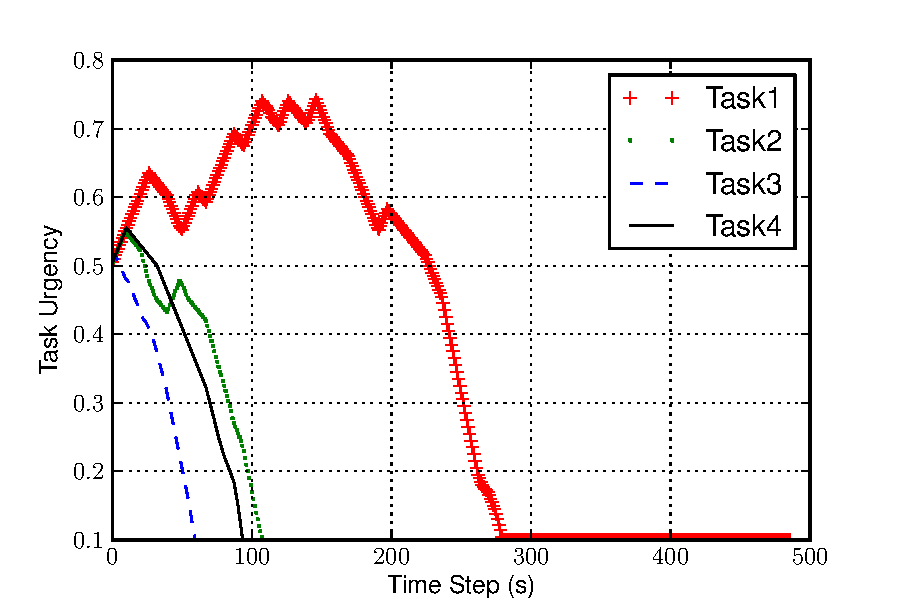
\includegraphics[width=7.5cm,height=5cm]{./images/PlotUrgencyLog-2010Feb15-171017}    % The printed column width is 8.4 cm.
\caption{Dynamic changes in task urgencies} 
\label{fig:task-urgency}
\end{center}
\end{figure}
%% 
\begin{figure}
\begin{center}
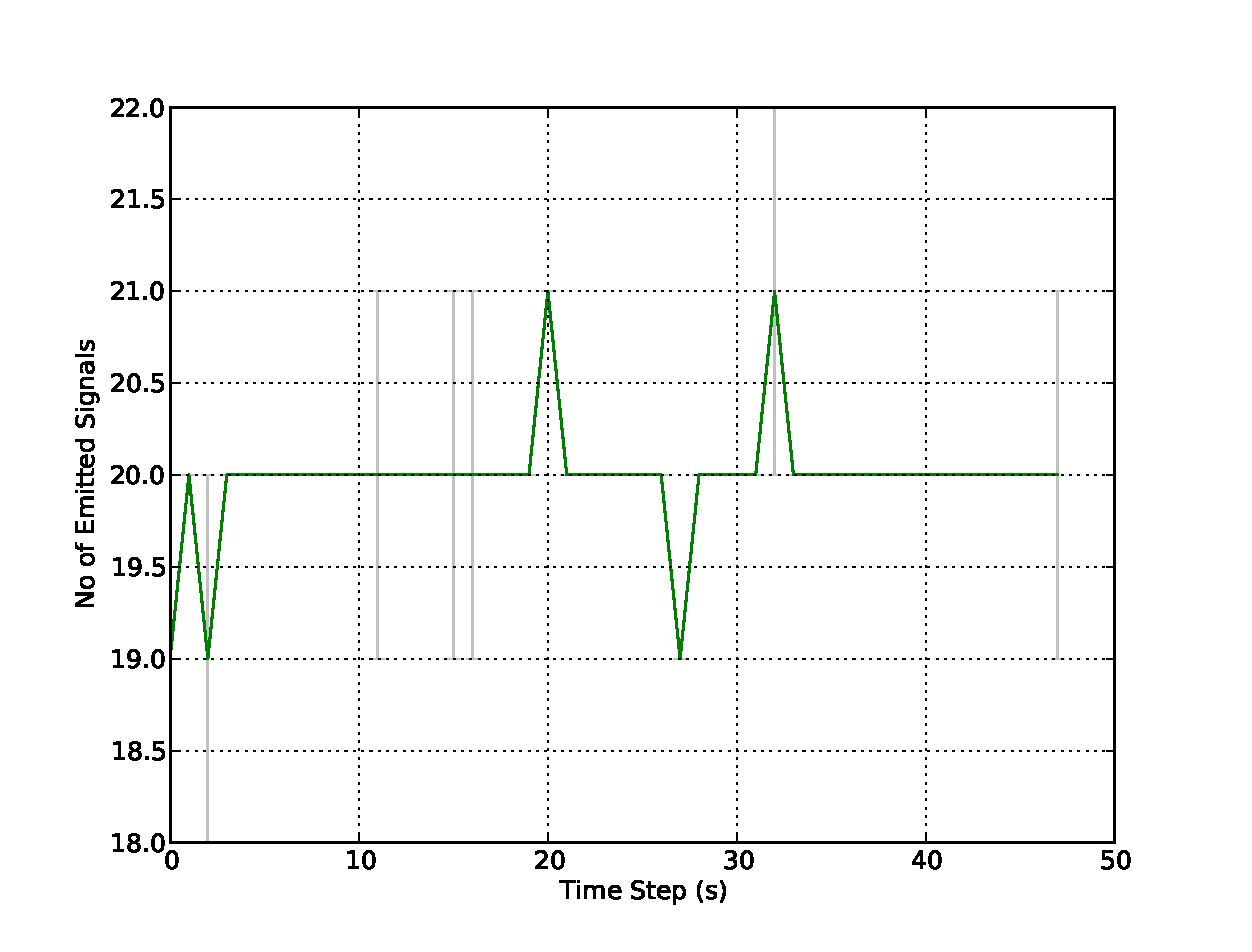
\includegraphics[width=7.5cm,height=5cm]{./images/Global-SignalingFreqStat}    % The printed column width is 8.4 cm.
\caption{D-Bus task information signalling frequency of TPA in centralized communication mode} 
\label{fig:global-freq}
\end{center}
\end{figure}
%%
\begin{figure}
\begin{center}
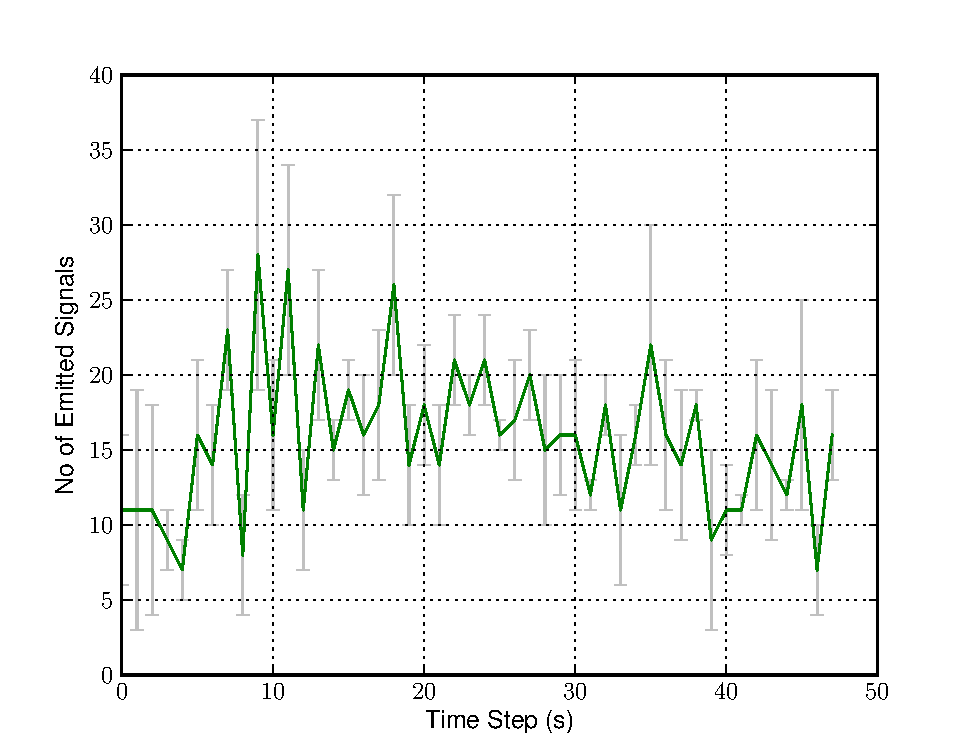
\includegraphics[width=7.5cm,height=5cm]{./images/Local-500cm-SignalingFreqStat}    % The printed column width is 8.4 cm.
\caption{D-Bus P2P task information signalling frequency of RCC of all robots in decentralized communication mode} 
\label{fig:local-freq}
\end{center}
\end{figure}
%% 
\begin{figure}
\begin{center}
%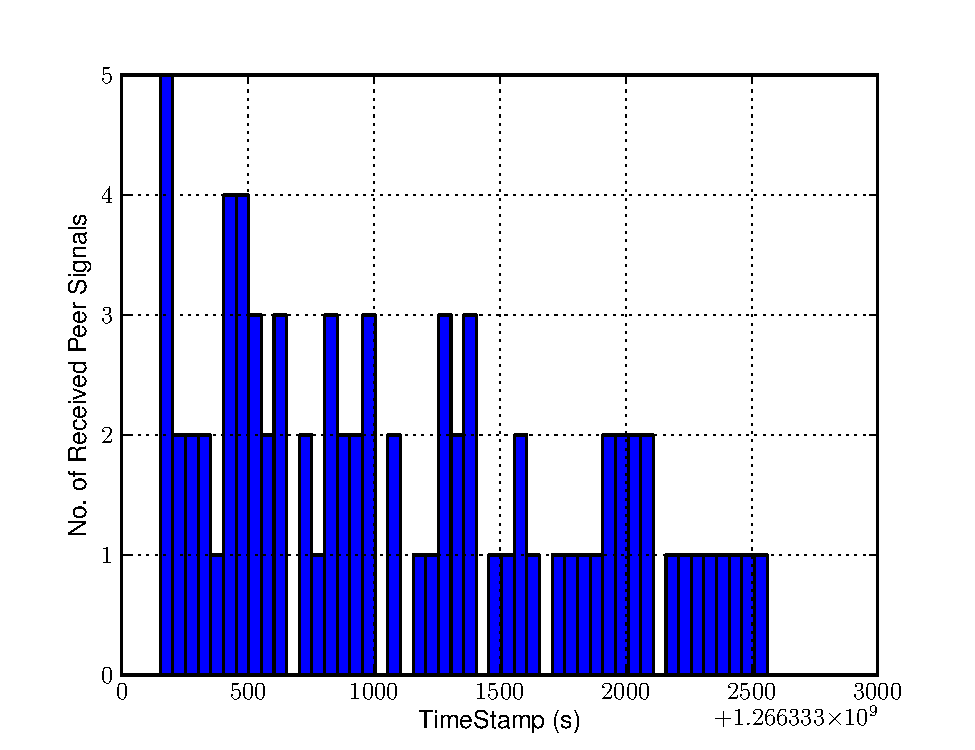
\includegraphics[width=7.5cm,height=5cm]{./images/Robot12-16feb-1-LocalSignals}     
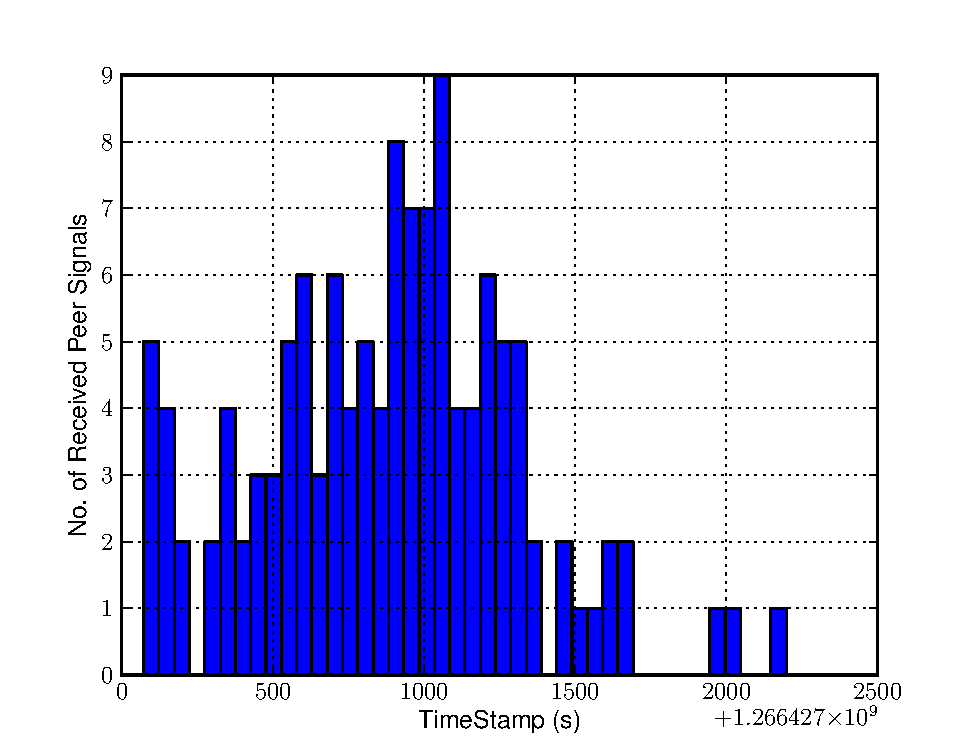
\includegraphics[width=7.5cm,height=5cm]{./images/Robot12-17feb-3-LocalSignals}
\caption{Robot12's simultaneous reception of D-Bus task information signals from peers} 
\label{fig:robot-freq}
\end{center}
\end{figure}
%===============================================================================
\section{Conclusion}
\label{sec:conc}
In this paper, we have presented a scalable hybrid multi-robot control architecture, hybrid event-driven architecture on D-Bus (HEAD), that relies on D-Bus inter-process communication technology. HEAD has several distinct differences from a classical hybrid architecture, e.g. being event-driven that makes sequencing task automated and robust, use of communication as sensing etc. From the architectural design and practical implementation in a MRS with 16 E-puck robots, we can say that HEAD is robust and scalable in terms of communication, sensing and control of various elements of a large MRS. We have achieved this, mainly, by decoupling the communication of heterogeneous software components into two separate processes of listening and emitting D-Bus signals.\\
Although \cite{Magnenat+2009} used D-Bus for managing control of different micro-controllers of a single robot, to our best of knowledge, in MRS literature there is no other instance of MRS that uses D-Bus in this fashion to control a large group of robots. In this regard, this work is a pioneering one in the field of multi-robot control. This same control strategy can be applied to many other fields, such as in multi-agent systems, networked control of different heterogeneous software components and so on. However, we need to extensively examine the performance of D-Bus with more components in much more complex tasks and environments. In future, we look forward to explore deploying HEAD in a MRS having about 40 E-puck robots.
%A conclusion section is not required. Although a conclusion may review the main points of the paper, do not replicate the abstract as the conclusion. A conclusion might elaborate on the importance of the work or suggest applications and extensions.

%\begin{ack}
%Place acknowledgments here.
%\end{ack}

\bibliography{control2010}             % bib file to produce the bibliography
                                                     % with bibtex (preferred)
                                                   
%\appendix
%\section{D-Bus Listener Code}    % Each appendix must have a short title.

%\section{D-Bus Emitter Code}              % Sections and subsections are supported  
                                                                         % in the appendices.
\end{document}